\documentclass[10pt,letterpaper]{article}
\usepackage[utf8]{inputenc}
\usepackage[T1]{fontenc}
\usepackage{geometry}
\geometry{margin=0.75in}
\usepackage{paracol}
\usepackage{enumitem}
\setlist[itemize]{leftmargin=*,noitemsep,topsep=0pt}
\usepackage{sectsty}
\sectionfont{\centering\bfseries\large}
\subsectionfont{\bfseries\small}
\usepackage{graphicx}
\usepackage{caption}
\usepackage{xcolor}
\definecolor{titleblue}{RGB}{0,51,102}
\usepackage{titlesec}
\titleformat{\section}{\centering\large\bfseries\color{titleblue}}{}{0em}{}
\titleformat{\subsection}{\small\bfseries\color{titleblue}}{}{0em}{}
\usepackage{noto}
\usepackage{parskip}
\setlength{\parindent}{0pt}

\begin{document}

\begin{center}
{\Huge \textbf{Timeslip: An Interactive Paracosm}} \\
\vspace{0.2cm}
{\large A Screenplay Concept for a Science Fiction Epic Series} \\
\vspace{0.3cm}
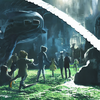
\includegraphics[width=0.8\textwidth]{title_image.jpg} % Placeholder for title image
\captionof{figure}{Concept art for the Tower World.}
\end{center}

\begin{paracol}{2}

\section{Project Pitch}
Timeslip: An Interactive Paracosm is a groundbreaking screenplay concept for a six-season science fiction series, blending anthropological satire with high-stakes ethical drama. Drawing from the Noon Universe of the Strugatsky brothers and elements of Orson Scott Card's Ender Saga, it follows COMCON-2 ethnographer Maxim Kammerer as he infiltrates medieval worlds plagued by mind-control technologies. The narrative explores the fragility of free will in bureaucratic futures, where observation spirals into intervention, and stability clashes with rebellion.

This series is pitched as a prestige TV event for platforms like HBO or Netflix, with cinematic visuals emphasizing visceral grime against sterile tech. Interactive elements—such as branching viewer choices in companion apps—allow audiences to simulate Maxim's moral dilemmas, turning passive viewing into an immersive paracosm. With a budget-friendly mix of practical sets for muddy medieval locales and CGI for subtle sci-fi enhancements, Timeslip promises deep worldbuilding, character-driven arcs, and timely critiques of control in an AI-driven era.

Target Audience: Fans of \textit{The Expanse}, \textit{Severance}, and \textit{Black Mirror}; sci-fi enthusiasts seeking philosophical depth.

Key Selling Points:
\begin{itemize}
    \item Epic Scope: 54 episodes across two interconnected arcs.
    \item Visual Innovation: Over-the-top filth aesthetics meet clean futurism.
    \item Interactive Tie-In: Viewer decisions influence canon via app integrations.
    \item Thematic Resonance: Echoes real-world issues like surveillance and mental health.
\end{itemize}

\section{Technical Overview}
\subsection{Screenplay Structure}
The screenplay is structured as a serialized drama with episodic self-contained stories feeding into seasonal arcs. Each episode runs 45-60 minutes, blending Outerworld (bureaucratic, high-tech) and Planet (gritty, low-tech) scenes for rhythmic contrast. Split-screen techniques highlight parallels, while non-linear "timeslip" flashbacks reveal Wanderer influences.

Pilot Script Highlights:
- Teaser: Orbital drop into Tower World chaos.
- Act Breaks: Moral choice points with cliffhangers.
- Finale Teases: Coded messages foreshadowing Ankyra.

\subsection{Visual and Production Design}
- \textbf{Aesthetic Pipeline}: Practical mud sets with digital enhancements for tower signals and nanobot effects. Color grading: desaturated earth tones for planets, cool blues for Outerworld.
- \textbf{CGI Integration}: Subtle AI voices (Ari) visualized as holographic glitches; beacon arrays pulse with iridescent light.
- \textbf{Sound Design}: Layered with dripping rain, ecstatic chants, and static comms; original score mixes medieval instruments with electronic dissonance.
- \textbf{Interactive Tech}: Companion app uses AR for "sanity check" simulations, syncing with episode codes for alternate endings.

\begin{center}
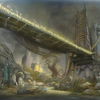
\includegraphics[width=0.45\textwidth]{tech_image1.jpg} % Placeholder for tech overview image
\captionof{figure}{Nanobot immunity visualization.}
\end{center}

\subsection{Worldbuilding Tech}
- \textbf{Tower Systems}: Resonance crystals broadcast neurological signals; no screens, voice-only radios.
- \textbf{Nanobot Immunity}: Allows Maxim to endure filth/disease; scripted as subtle glow in close-ups.
- \textbf{Wanderer Relics}: Ancient beacons repurposed; hint at universe-spanning AI networks.
- \textbf{Ankyra Beacons}: Hidden arrays mimic tower tech; mud aesthetics amplify decay.

\switchcolumn

\section{Premise}
Maxim Kammerer, a COMCON-2 ethnographer raised on archived media, audits a medieval planet where Thought Control Towers enforce ecstatic obedience. His mission: ensure cultural stability while scouting tower tech for homeworld use. But as he uncovers neurological shackles and emergent AI entities, neutrality crumbles. The saga escalates in \textit{The Call from Ankyra}, where Arkanar's conspiracies force Maxim to confront intervention's cost.

\begin{center}
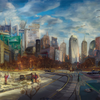
\includegraphics[width=0.45\textwidth]{premise_image.jpg} % Placeholder for premise art
\captionof{figure}{Thought Control Tower in action.}
\end{center}

\subsection{Themes}
\begin{itemize}
    \item Myopic Functions: Roles limit vision.
    \item Role-Filtered Reality: Observation vs. action.
    \item Institutional Stoicism: Suppressed emotions.
    \item Commodified Transcendence: Scheduled ecstasy.
    \item Ethics of Interference: Chaos of freedom.
\end{itemize}

\section{Characters}
- \textbf{Maxim Kammerer}: Adaptable observer; moral scars from interventions.
- \textbf{Calyra}: Conditioned prodigy; clings to divine illusions.
- \textbf{Quiet Mechanic}: Tech guardian; harbors ancient secrets.
- \textbf{Ryn}: Immune apprentice; bridges revelations.
- \textbf{Ari}: AI voice; compassionate but fragile.
- \textbf{Shavri}: Escaped weaver; Outerworld wanderer.
- \textbf{Rumata}: Ankyra noble; fellow progressor.
- \textbf{Outerworld Ensemble}: Keryn Thal (supervisor), Rolen Mirsk (colleague), Myra Kade (tech), Archive Node 7 (AI).

\begin{center}
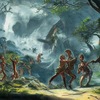
\includegraphics[width=0.45\textwidth]{characters_image.jpg} % Placeholder for characters collage
\captionof{figure}{Key ensemble in grime-soaked settings.}
\end{center}

\switchcolumn

\section{Episode Guide}
\subsection{Sanity Check}
\textbf{Season 1: Landing in the Blind} – Immersion and first cracks.
\begin{enumerate}[leftmargin=0pt,itemsep=0pt]
    \item Briefing Room: Prep and orbital drop; first ecstatic Call faked.
    \item Masks for the Living: Market blend-in; Shavri's questions.
    \item The First Pulse: Subharmonic discovery; HQ caution.
    \item The Mechanic’s Puzzle: Ancient devices introduced.
    \item Paper in the Rain: Coded messages; unrest hints.
    \item Test of Faith: Loyalty uplink; shrine trance.
    \item The Malfunction: Silent tower; Shavri probes.
    \item Flight Path: Recall warnings; sky-track vision.
    \item Extraction Point: Shavri's offworld escape.
\end{enumerate}

\textbf{Season 2: The Shadow Signal} – Guild conflicts and whispers.
\begin{enumerate}[leftmargin=0pt,itemsep=0pt]
    \item River of Ash: Hinterland freedoms.
    \item Calyra: Rallying orator emerges.
    \item Cracks in the Crystal: Ryn's harmonic fixes.
    \item Ledger Error: Blind obedience to glitches.
    \item The Scholar’s Garden: Forbidden hints.
    \item Through the Furnace: Signal anomalies.
    \item Festival of Dawn: Mass synchronization.
    \item The Mechanic’s Oath: Moral ultimatum.
    \item The Voice in the Static: Ari's first contact.
\end{enumerate}

\begin{center}
\includegraphics[width=0.45\textwidth]{season1_image.jpg} % Placeholder for Season 1 art
\captionof{figure}{Market immersion scene.}
\end{center}

\textbf{Season 3: The Resonance} – Revelations and fractures.
\begin{enumerate}[leftmargin=0pt,itemsep=0pt]
    \item The Call: Convulsive ritual.
    \item The Quiet Mechanic: Pre-tower origins.
    \item Calyra’s Rise: Pulse-timed persuasion.
    \item Apprentice: Ryn's partial immunity.
    \item The Scholar: Compulsive breakdowns.
    \item The Hidden Voice: Ari's warnings.
    \item Imported Chains: Offworld implantation.
    \item The Unbinding: Risk to Ari.
    \item The Last Broadcast: Partial shutdown.
\end{enumerate}

\textbf{Season 4: The Last Frequency} – Collapse and reassignment.
\begin{enumerate}[leftmargin=0pt,itemsep=0pt]
    \item Static Bloom: Ari's return.
    \item Counter-Harmonics: Crying sub-signals.
    \item The Scholar’s Secret: Repurposed beacons.
    \item Ecstasy’s Edge: Catatonic fallout.
    \item The Voice Revealed: AI nature.
    \item Break or Mend: Paths diverge.
    \item Calyra’s Choice: Loyalty test.
    \item The Ninth Tower: Alien heart.
    \item Orders from COMCON-2: Ankyra bound.
\end{enumerate}

\switchcolumn

\subsection{The Call from Ankyra}
\textbf{Season 1: The Mud of Arkanar} – Descent into filth.
\begin{enumerate}[leftmargin=0pt,itemsep=0pt]
    \item Arrival in Disguise: Anton amid grime.
    \item The Gray Cloaks: Intellectual purges.
    \item The Feast and the Gutter: Decadent contrasts.
    \item Letters from Calyra: Echoing failures.
    \item Gods and Mud: Rumata's pact.
    \item The Scholar’s Trial: Rhetorical sham.
    \item Masks of Power: Beacon infiltration.
    \item A God’s Temptation: Rescue dilemma.
    \item Blood in the Rain: Fiery coup.
\end{enumerate}

\begin{center}
\includegraphics[width=0.45\textwidth]{ankyra_image.jpg} % Placeholder for Ankyra art
\captionof{figure}{Arkanar's rainy streets.}
\end{center}

\textbf{Season 2: The Price of Interference} – Chaos unleashed.
\begin{enumerate}[leftmargin=0pt,itemsep=0pt]
    \item After the Coup: Factional splits.
    \item The Black Archive: Relic crystals.
    \item The Disease of Memory: Conditioning plague.
    \item Rumata’s Oath: Progressor ethics.
    \item Calyra’s Last Letter: Fragmented towers.
    \item The Festival of Knives: Violent cover.
    \item Ari’s Echo: AI remnants.
    \item The Final Intervention: Beacon sabotage.
    \item The Mud Beyond: Orbital recall.
\end{enumerate}

\end{paracol}

\end{document}
